\documentclass[12pt]{elsarticle}
\usepackage[bottom=2cm,top=3cm,left=3cm,right=2cm]{geometry}
\usepackage{url}
\makeatletter
\def\ps@pprintTitle{%
      	\let\@oddhead\@empty
      	\let\@evenhead\@empty
      	\def\@oddfoot{\reset@font\hfil\thepage\hfil}
      	\let\@evenfoot\@oddfoot
}
\makeatother

\usepackage{babelbib}

\usepackage[brazilian]{babel} % Traduz alguns termos para o português
\usepackage[utf8]{inputenc} % Reconhece acentuação
\usepackage{setspace}

\onehalfspacing

\begin{document}

	\begin{frontmatter}

		\title{ELE083 Computação Evolucionária\\ \resizebox{7cm}{0.3cm}{Laboratório II - Problema da Mochila}}
		\author{Davi Pinheiro Viana - 20130229912\\Rafael Carneiro de Castro - 2013030210}
		\address{Minas Gerais, Brasil}
		
		\begin{keyword}
			Computação Evolucionária\sep Algoritmos genéticos \sep Problema da Mochila
		\end{keyword}
	\end{frontmatter}
	
	\section{Introdução}
	O objetivo do trabalho é resolver o problema da mochila utilizando o \emph{Algoritmo Genético Geracional (GGA)} e, variando o valor da probabilidade de mutação $p_m$ e da probabilidade de cruzamento $p_c$, analisar o efeito desses parâmetros no desempenho do algoritmo.

	\section{Influência dos parâmetros no desempenho do algoritmo}
	A primeira análise feita para verificar os efeitos da influência dos parâmetros no desempenho do algoritmo foi considerar uma execução em que não ocorre cruzamentos e outra em que não ocorre mutações, segue, abaixo, o resultado:
	\begin{figure}[h]
		\centering
		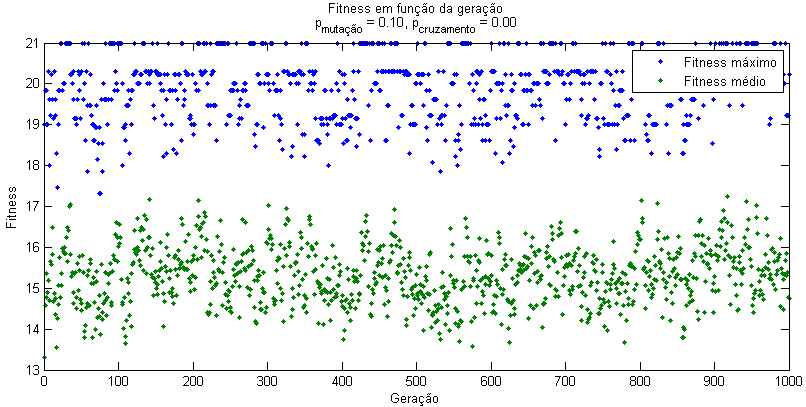
\includegraphics[width=15cm]{img/pc_0.png}
		\caption{Resultado do algoritmo para $p_{c}=0$}
		\label{fig:pc_0}
	\end{figure}
	
	\begin{figure}[h]
		\centering
		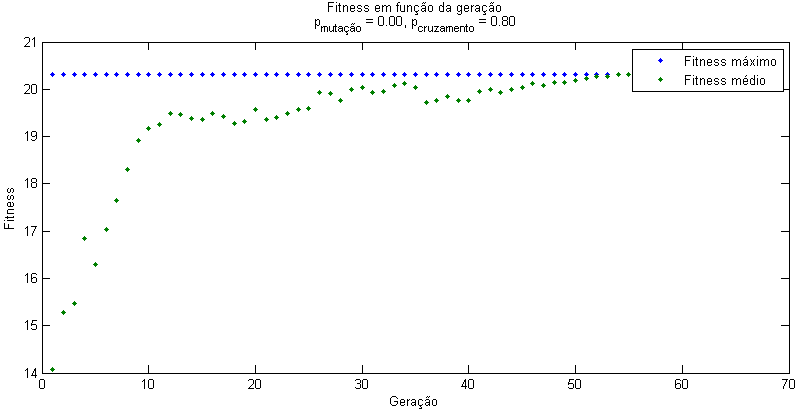
\includegraphics[width=17cm]{img/pm_0.png}
		\caption{Resultado do algoritmo para $p_{m}=0$}
		\label{fig:pm_0}
	\end{figure}
	
	A partir das figuras \ref{fig:pc_0} e \ref{fig:pm_0}, pode-se observar que o valor da probabilidade de mutação interfere bem mais no resultado do que o valor da probabilidade de cruzamento.
	
	Sem mutação, não há muita variabilidade na população ao longo das gerações, mesmo ocorrendo cruzamento, por isso o algoritmo convergiu rapidamente para um determinado valor de função de aptidão tanto para valores máximos quanto para médios da mesma, como mostra a Figura \ref{fig:pm_0}.
	
	Enquanto que, para o caso onde não temos cruzamento, obtemos variabilidade só por termos mutação. Podemos ver pela Figura \ref{fig:pc_0} que o algoritmo até consegue manter o melhor indivíduo por algumas gerações (valor de aptidão máximo do melhor indivíduo igual a 21), mas perde esse valor devido às mutações e também ao tipo de algoritmo.
	
	A segunda análise feita foi considerando dois cenários: o primeiro em que sempre ocorre mutação ($p_m=1$) e o segundo em que sempre ocorre cruzamento ($p_c=1$). Segue, abaixo, o resultado:
	\newpage
	\begin{figure}[h]
		\centering
		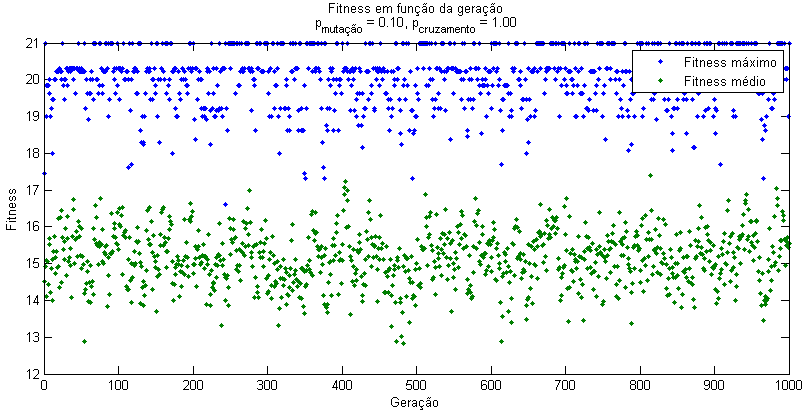
\includegraphics[width=13cm]{img/pc_1.png}
		\caption{Resultado do algoritmo para $p_{c}=1$}
		\label{fig:pc_1}
	\end{figure}
	
	\begin{figure}[h]
		\centering
		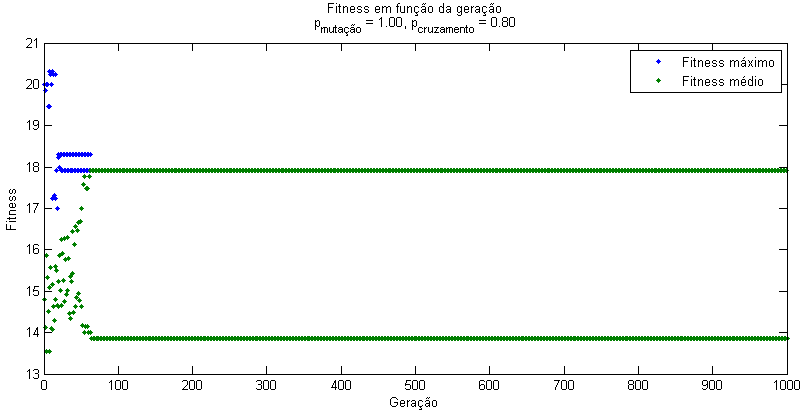
\includegraphics[width=13cm]{img/pm_1.png}
		\caption{Resultado do algoritmo para $p_{m}=1$}
		\label{fig:pm_1}
	\end{figure}
	
	A partir das figuras \ref{fig:pc_0} e \ref{fig:pc_1} pode-se notas que não há muita diferença nas formas de ambas as curvas, o que indica que mesmo ocorrendo cruzamento em todas as gerações sempre, não temos muita influência, pelo menos desse tipo de cruzamento, gerada pela sua ocorrência no algoritmo.
	Na Figura \ref{fig:pm_1}, percebemos, que ocorrendo mutação sempre, a variabilidade se torna tão grande que o algoritmo não consegue manter o melhor indivíduo.
	\newpage
	A terceira e última análise feita para analisar o efeito dos parâmetros foi aumentar progressivamente os parâmetros e analisar o efeito. Segue, abaixo, o resultado:
	\begin{figure}[h]
		\centering
		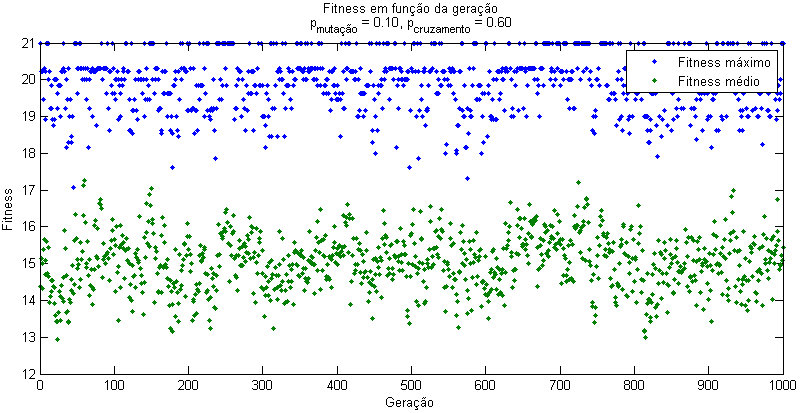
\includegraphics[width=13cm]{img/pc_06.png}
		\caption{Resultado do algoritmo para $p_{c}=0,6$}
		\label{fig:pc_06}
	\end{figure}
	
	\begin{figure}[h]
		\centering
		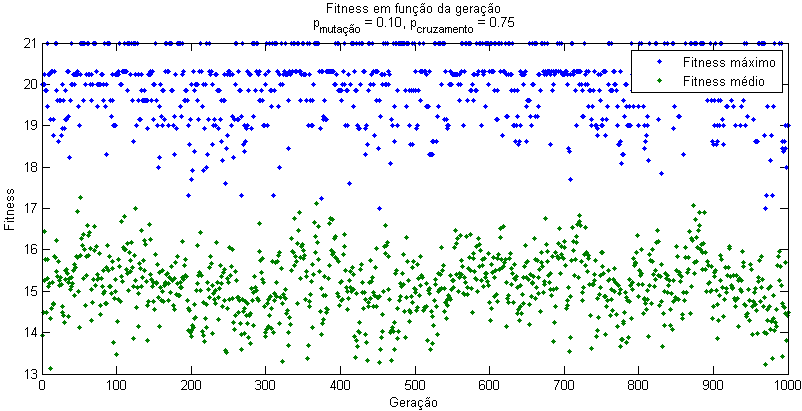
\includegraphics[width=13cm]{img/pc_075.png}
		\caption{Resultado do algoritmo para $p_{c}=0,75$}
		\label{fig:pc_075}
	\end{figure}
	\newpage
	
	\begin{figure}[h]
		\centering
		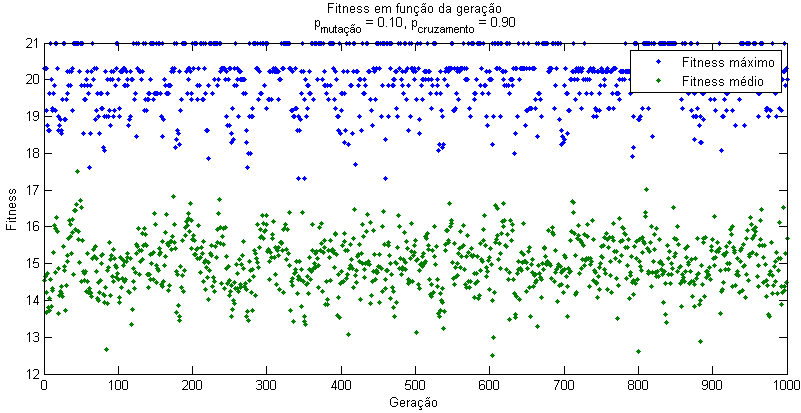
\includegraphics[width=13cm]{img/pc_09.png}
		\caption{Resultado do algoritmo para $p_{c}=0,9$}
		\label{fig:pc_09}
	\end{figure}
	
	\begin{figure}[h]
		\centering
		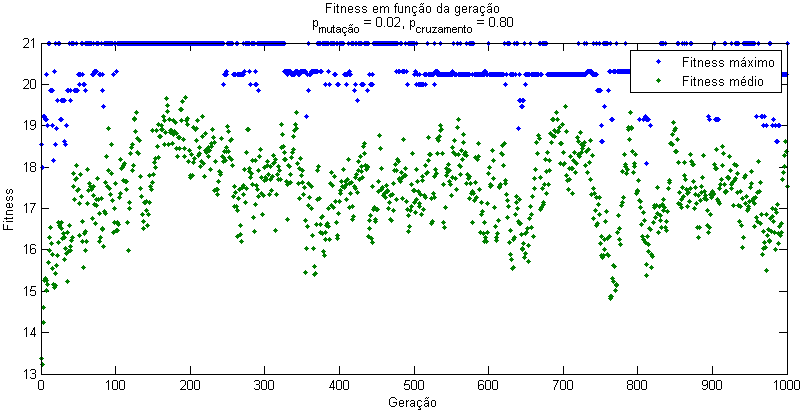
\includegraphics[width=13cm]{img/pm_002.png}
		\caption{Resultado do algoritmo para $p_{m}=0,02$}
		\label{fig:pm_002}
	\end{figure}
	
	\newpage
	\begin{figure}[h]
		\centering
		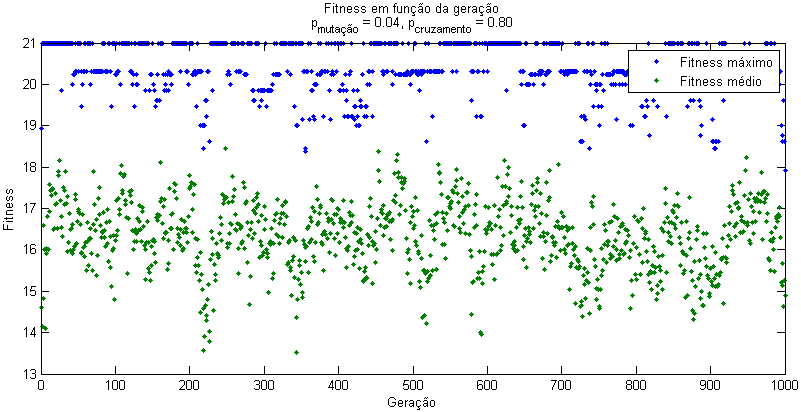
\includegraphics[width=13cm]{img/pm_004.png}
		\caption{Resultado do algoritmo para $p_{m}=0,04$}
		\label{fig:pm_004}
	\end{figure}
	
	\begin{figure}[h]
		\centering
		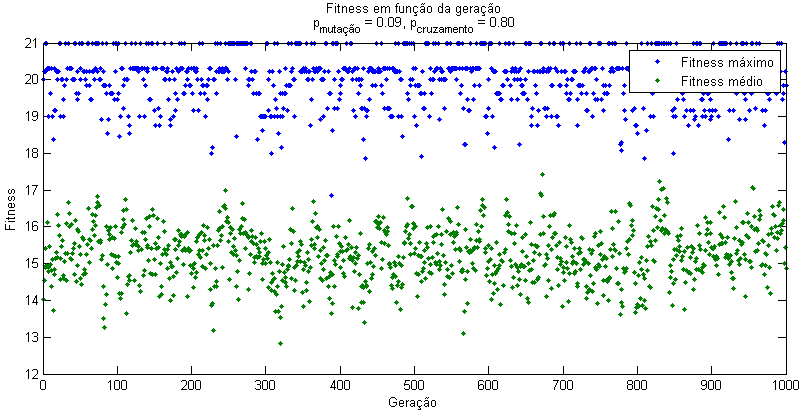
\includegraphics[width=13cm]{img/pm_009.png}
		\caption{Resultado do algoritmo para $p_{m}=0,09$}
		\label{fig:pm_009}
	\end{figure}
	\newpage
	\begin{figure}[h]
		\centering
		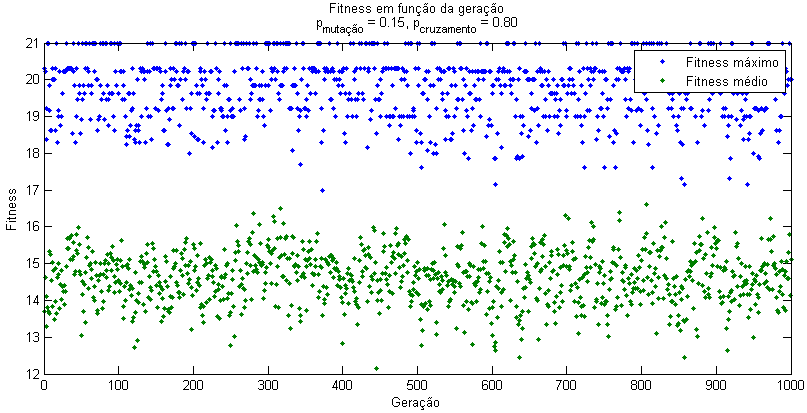
\includegraphics[width=13cm]{img/pm_015.png}
		\caption{Resultado do algoritmo para $p_{m}=0,15$}
		\label{fig:pm_015}
	\end{figure}
	
	A partir das figuras \ref{fig:pc_06}, \ref{fig:pc_075} e \ref{fig:pc_09} pode-se concluir que, mantendo um valor de $p_m$ fixo, a forma da curva de aptidão média se mantém e quanto maior $p_c$ mais vezes o melhor indivíduo é mantido, devido a ocorrência de mais cruzamentos e maior variabilidade relacionada ao mesmo sendo acrescentada à de mutação.
	
	A partir das figuras \ref{fig:pm_002}, \ref{fig:pm_004}, \ref{fig:pm_009} e \ref{fig:pm_015}, desta vez mantendo $p_c$ fixo, quanto menor $p_m$, por mais gerações o algoritmo mantém o melhor indivíduo, isso porque os valores se aproximam de $p_m = 0$, onde temos cada vez mais influência de $p_c$ que como vimos, neste caso não é muito grande.
	Os valores de aptidão média nessas figuras parecem convergir mais ao aumentar $p_m$, mostrando que apesar do algoritmo não convergir para um determinado valor fixo, por causa da técnica de seleção dos sobreviventes de substituição baseada em idade, adotada pelo \emph{GGA}, o mesmo consegue convergir, concentrando os valores tanto de aptidão máxima como média em um intervalo, a medida que temos variabilidade tanto devido ao cruzamento quanto à mutação.

\end{document}